% \begin{figure}[t]
%     \centering
%     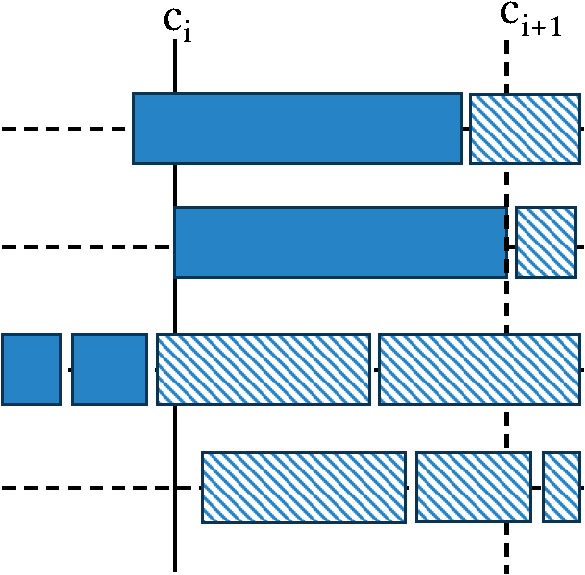
\includegraphics[width=0.6\linewidth]{figs/f1-crop.pdf}
%     \caption{\small{\textbf{Advancing global clock in SCRR.}}}
% 	\label{fig:global-clock}
% \end{figure}

% \begin{figure}[t]
%     \centering
%     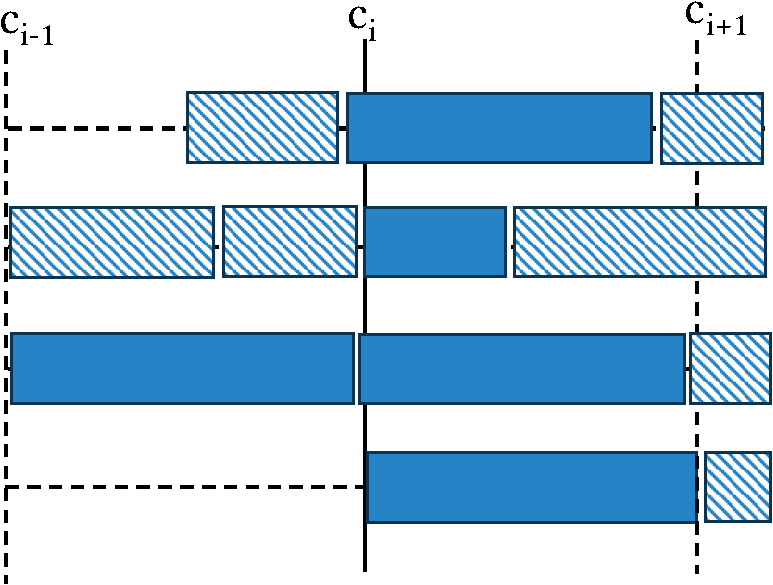
\includegraphics[width=0.6\linewidth]{figs/f2-crop.pdf}
%     \caption{\small{\textbf{Advancing the sub-queue clock in SCRR.}}}
% 	\label{fig:local-clock}
% \end{figure}

\begin{figure}[t]
    \centering
    \vspace{3mm}
    \begin{subfigure}[t]{.46\linewidth}
        \centering
        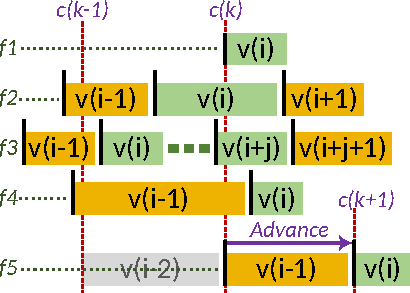
\includegraphics[width=1\linewidth]{figs/scrr-packet-advance-start.pdf}
        \caption{\small{\textit{Advancing global clock}}}
    	\label{fig:global-clock-start}
    \end{subfigure}
    \rulesep
    \begin{minipage}{.50\linewidth}
        \vspace{-20mm}
        \centering
	\begin{subfigure}[t]{1.0\linewidth}
            \centering
            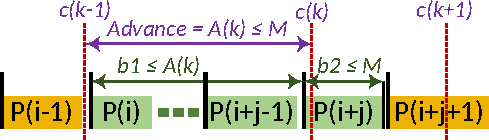
\includegraphics[width=1\linewidth]{figs/scrr-packet-burst-start.pdf}
            \vspace{-6mm}
            \caption{\small{\textit{Maximum burstiness}}}
	    \label{fig:burstiness-start}
	\end{subfigure}\\
        \vspace{1mm}
	\begin{subfigure}[t]{0.9\linewidth}
            \centering
            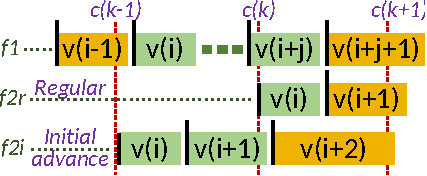
\includegraphics[width=1\linewidth]{figs/scrr-initial-advance-start.pdf}
            \vspace{-6mm}
            \caption{\small{\textit{Initial Advance}}}
	    \label{fig:initial-advance-start}
	\end{subfigure}
    \end{minipage}\\
    \vspace{-4mm}
    \caption{\small{SCRR clock management with start-time semantics.}}
    \label{fig:scrr-start}
    \vspace*{-0.4cm}

    % \hspace{10pt}
\end{figure}

% \begin{figure}[t]
%     \centering
%     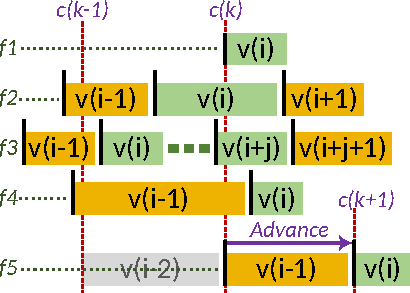
\includegraphics[width=0.6\linewidth]{figs/scrr-packet-advance-start.pdf}
%     \caption{\small{\textbf{Advancing global clock in SCRR with start-time.}}}
% 	\label{fig:global-clock-start}
% \end{figure}

% \begin{figure}[t]
%     \centering
%     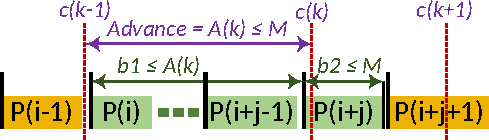
\includegraphics[width=0.6\linewidth]{figs/scrr-packet-burst-start.pdf}
%     \caption{\small{\textbf{Burstiness of SCRR with start-time.}}}
% 	\label{fig:burstiness-start}
% \end{figure}
